\chapter{THE CMS DETECTOR} 
\label{ch:cms_detector}
%%%%%%%%%%%%%%%%%%%%
\begin{figure}[pbth]
\centering
\includegraphics[width=10cm,height=10cm,keepaspectratio]{figures/cms/cms_poster_SX5.jpg}
    \caption{
    Life-size poster of the CMS detector, taken during CERN Open Days 2019
    in the SX5 warehouse where parts of CMS were assembled.}
    \label{fig:cms_poster}
\end{figure}
%%%%%%%%%%%%%%%%%%%%
Weighing in at 14,000 tonnes, standing 5 stories tall (15 m), and reaching 29 m long, the Compact Muon Solenoid (CMS) experiment is one of two general-purpose particle detectors at the LHC (Fig.~\ref{fig:cms_poster}).
CMS is situated approximately 100 m under the earth at the fifth collision point (Point 5) along the LHC (Fig.~\ref{fig:lhc_points}).
In 2012, both CMS and its competing experiment, ATLAS, independently discovered the Higgs boson.

% The purpose of CMS is to precisely measure the kinematical properties of the abundant decay products that come from the \pp collisions delivered by the LHC.
% These particle properties, like momentum, energy, and charge, are used to reconstruct the particle trajectories (``tracks'') and help to identify the particles themselves.
As discussed in Section (TODO: REF), the LHC collides bunches of protons every 25 ns to produce thousands of new particles which then travel away from the interaction point.
CMS is built around the interaction point in a series of cylindrical subdetectors for nearly hermetic coverage so that most of the particles must travel through CMS.
The detector sports a solenoid, after which CMS was named, which generates a 3.8 T uniform magnetic field that points longitudinally down the central axis of CMS.
This strong magnetic field applies a Lorentz force on the outgoing charged particles, causing them to follow helical, momentum-dependent trajectories.
These curved tracks are then better separated from one another which assists in particle identification.
Neutral particles experience no Lorentz force and thus travel in straight lines.

The subdetectors measure the properties of the outgoing particles and carefully filter them out in a clever way (Fig.~\ref{fig:cms_cut_out_view}).
Particles interact with the subdetectors, leaving so called ``hits'' where they passed through.
% As the particles interact with the subdetectors in CMS, they leave leaving indication that 
Hits are reconstructed into tracks.
From the track curvature, deduce charge and momentum of the particles.
Depending on which subdetector (or combination of subdetectors) was hit by the outgoing particles, the type of particle can be deduced.
%%%%%%%%%%%%%%%%%%%%
\begin{figure}[pbth]
\centering
\includegraphics[width=13cm,height=13cm,keepaspectratio]{figures/lhc/lhc_points_with_buildings.png}
    \caption{
    Points 1 through 8 along the LHC.
    Collisions occur at 
    Points 1 (ATLAS), 2 (ALICE), 5 (CMS), and 8 (LHCb),
    whereas the remaining points are used for LHC beam maintenance and testing.} 
    \label{fig:lhc_points}
\end{figure}
%%%%%%%%%%%%%%%%%%%%
%%%%%%%%%%%%%%%%%%%%
\begin{figure}[pbth]
\centering
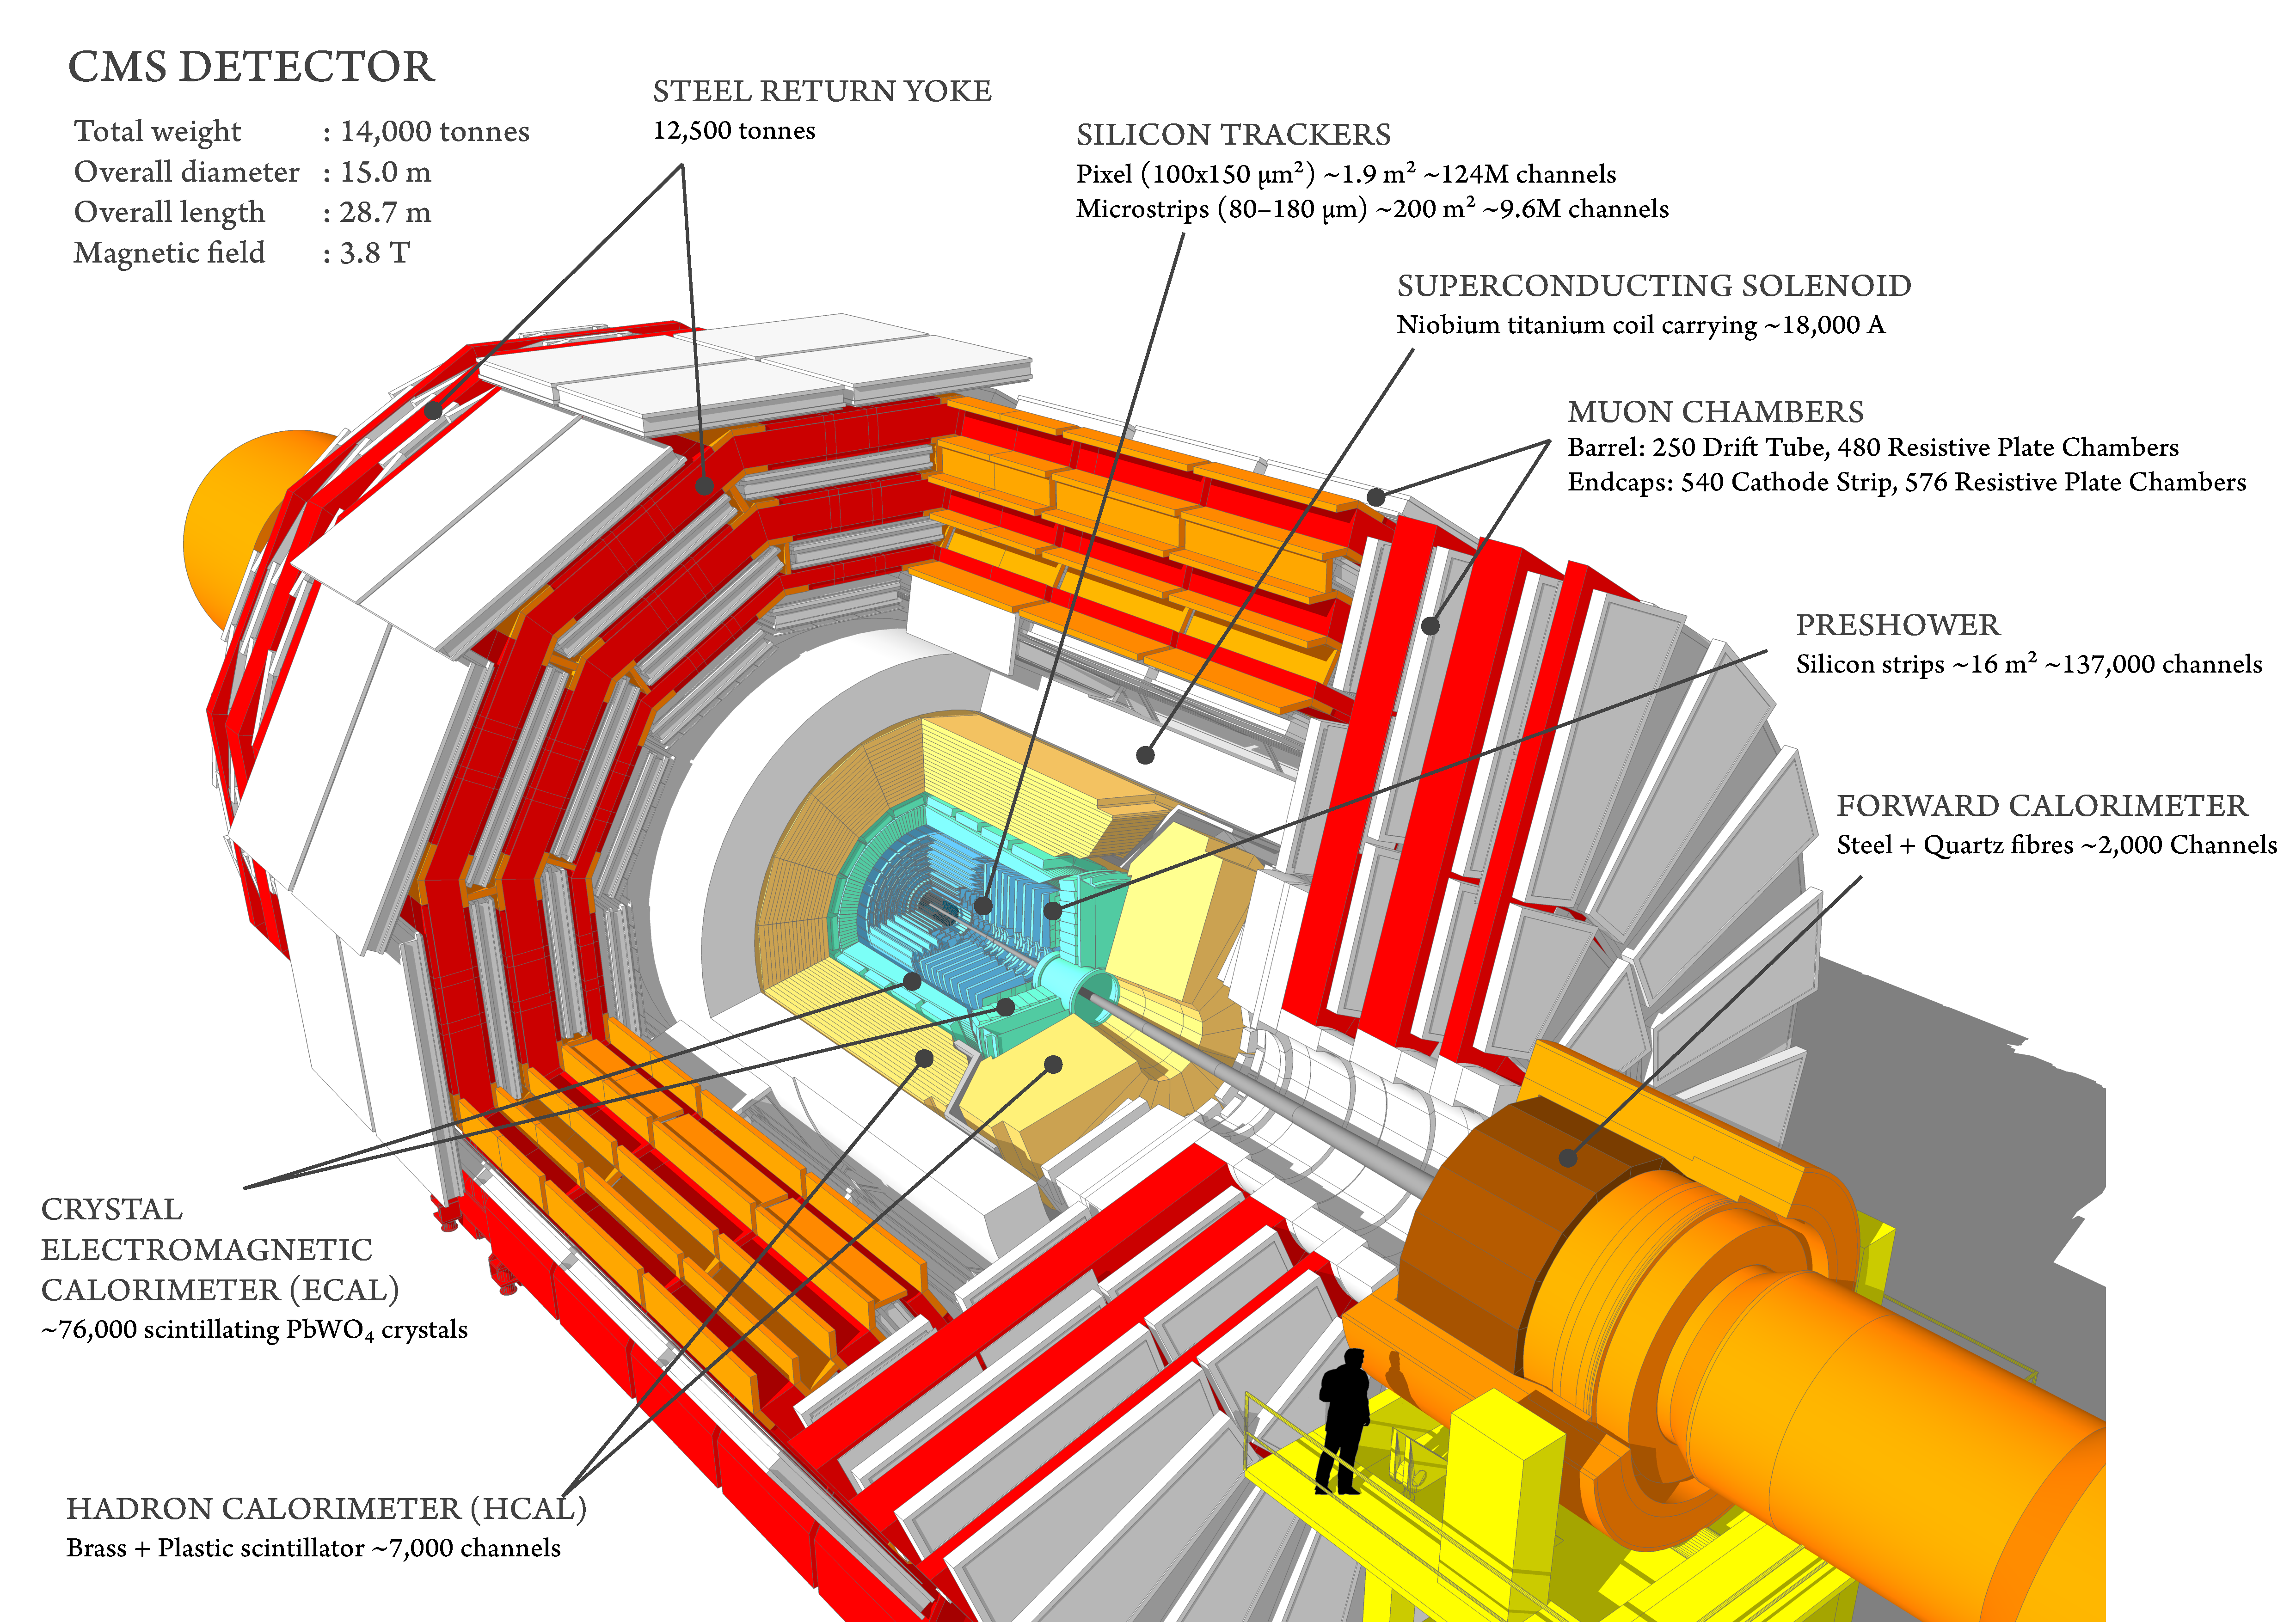
\includegraphics[width=15cm,height=15cm,keepaspectratio]{figures/cms/cms_cut_away.png}
    \caption{Cut out of the CMS detector showing its various subdetector components.} 
    \label{fig:cms_cut_out_view}
\end{figure}
%%%%%%%%%%%%%%%%%%%%
A few example particles and their associated tracks are shown in Fig.~\ref{fig:cms_particle_trajectories}.

Before discussing each subdetector in the following sections, it is useful to define the coordinate system used in CMS:
a typical, right-handed, three-dimensional Cartesian coordinate system $(x, y, z)$ is used, whose center $(0, 0, 0)$ is placed at the nominal \pp collision point within CMS.
The $x$-axis points towards the center of the LHC, the $y$-axis points vertically upward, and the $z$-axis points westward towards the Jura mountains, tangential to the beam direction.
Since CMS covers almost the entire spherical $4\pi$ steradians around the interaction point, it is convenient to use spherical coordinates $(r, \phi, \theta)$,
in which $r$ measures the radial distance in the $x$-$y$ plane, $\phi$ measures the azimuthal angle in the $x$-$y$ plane as measured from the $x$-axis, and $\theta$ measures the polar angle as measured from the $z$-axis.
When dealing with ultra-relativistic particles like those produced at the LHC, special relativistic effects like length contraction must be taken into account and so the coordinate $\theta$ becomes frame-dependent.
It is thus helpful to convert $\theta$ to the Lorentz-invariant quantity called pseudorapidity $(\eta)$,
defined as $\eta = -\ln [ \tan(\theta/2)]$. % Formula comes from: https://twiki.cern.ch/twiki/bin/view/Sandbox/GeorgeAlversonSandbox#Symbols_and_units_natural_units
% \begin{equation*}
%     \eta = -\ln \left(
%         \tan (\theta / 2)
%         \right)
% \end{equation*}
% which surround the 
%%%%%%%%%%%%%%%%%%%%
\begin{figure}[pbth]
\centering
\includegraphics[width=15cm,height=15cm,keepaspectratio]{figures/cms/cms_transverse_particletrajectories_corrected.png}
    \caption{
    A transverse view of CMS showing the ``filtration process'' as different particles pass through different subdetectors.
    A positron (solid red line) curves due to the presence of the magnetic field and gets stopped in the ECAL, creating an EM shower.
    A photon (blue dashed line) does not get detected at all by the Silicon Tracker, since it has no electric charge.
    It continues through to the ECAL and makes a shower here, like the positron.
    Charged hadrons (solid green line) will show curved tracks from the Silicon Tracker, may leave some trace in the ECAL, but primarily get stopped by the HCAL creating hadronic showers.
    Neutral hadrons (dashed green line) do not interact with the tracker, and only undergo EM showers a little in the ECAL, but show most energy deposits in the HCAL.
    Muons (solid blue line) are detected by the Silicon Tracker and then mostly pass through the other subdetectors without interacting until they finally reach the Muon System.
    % In fact you can even determine whether its charge is positive or negative since
    % q v cross B gives the direction of Force.
    % The velocity of the muon is out like this, and the B field is into the screen, so the applied force would be up like this for a positive particle. 
    Using the Lorentz force law and knowing which direction the magnetic field is pointing, one can deduce the sign of the charge of the particle. 
    Based on the radius of curvature from the trajectory, one can then calculate the momentum and energy of the particle.
    % We see that it's not curving up, but curving the other way so we know it must be negative.
    % Notice that since it is curving the opposite way from the muon so we know this is a positive particle.
    % Next up the solid green trajectory represents a charged hadron, like for example maybe an antiproton that got produced.
    % Notice that it would be the same sign as the muon because they curve in the same direction.
    } 
    \label{fig:cms_particle_trajectories}
\end{figure}
%%%%%%%%%%%%%%%%%%%%
% After the protons collide, they make a mess of all sorts of particles:
% electrons, lambda baryons, kaons, muons, photons...